\pagebreak
\section{Procesos}
\begin{itemize}
    \item Programa en ejecucion.
    \item \textbf{Programa:}
        \begin{itemize}
            \item Es estacico.
            \item No tiene program counter.
            \item Existe desde que se edita hasta que se boora.
        \end{itemize}
    \item \textbf{Proceso:}
        \begin{itemize}
            \item Es dinamico.
            \item Tiene program counter.
            \item Su ciclo de vida comprende desde que se solicita ejecutar hasta que termina.
        \end{itemize}
\end{itemize}

\subsection{Atributos de un proceso}
\begin{itemize}
    \item Identificaion del proceso y del proceso padre.
    \item Identificacion del usuario que lo disparo.
    \item Si hay estructura de grupos, grupo que lo dispario.
    \item En ambientes multiusuario, desde que terminal y quien lo ejecuto.
\end{itemize}

\subsection{Componentes de un proceso}
\begin{itemize}
    \item Seccion de codigo.
    \item Seccion de Datos.
    \item Stack(s): Datos temporarios.
\end{itemize}

\subsection{Process Control Block (PCB)}
\begin{itemize}
    \item Estructura de datos asociada al proceso (abstraccion).
    \item Existe una por proceso.
    \item Es lo primero que se crea cuando se crea un proceso y lo ultimo que se borra cuando termina.
    \item Contiene la informacion asociada con cada proceso:
        \begin{itemize}
            \item PID, PPID, etc.
            \item Valores de los registros de la CPU.
            \item Planificacion.
            \item Ubicacion en memoria.
            \item Accounting.
            \item Entrada/Salida.
        \end{itemize}
\end{itemize}

\subsubsection{Stacks}
\begin{itemize}
    \item Un proceso cuenta con 1 o mas stacks.
    \item Se crean automaticamente y su medida se ajusta en run-time.
    \item Esta formado por stack frames que son pushed (al llamar una rutina) y popped (cuando se retorna de ella).
    \item el stack frametiene los parametros de la rutina y los datos necesarios para recuperar el stack frame anterios.
\end{itemize}

\subsection{Espacio de direcciones de un proceso}
\begin{itemize}
    \item Conjunto de direcciones de memoria que ocupa el proceso.
    \item No incluye su PCB o tablas asociadas.
    \item Un proceso en modo usuario solo puede acceder a su espacio de direcicones.
    \item En modo Kernel, se puede acceder a estructuras internas (PCB del proceso) o a espacio de direcciones de otros procesos.
\end{itemize}
\begin{figure}[ht]
    \begin{center}
        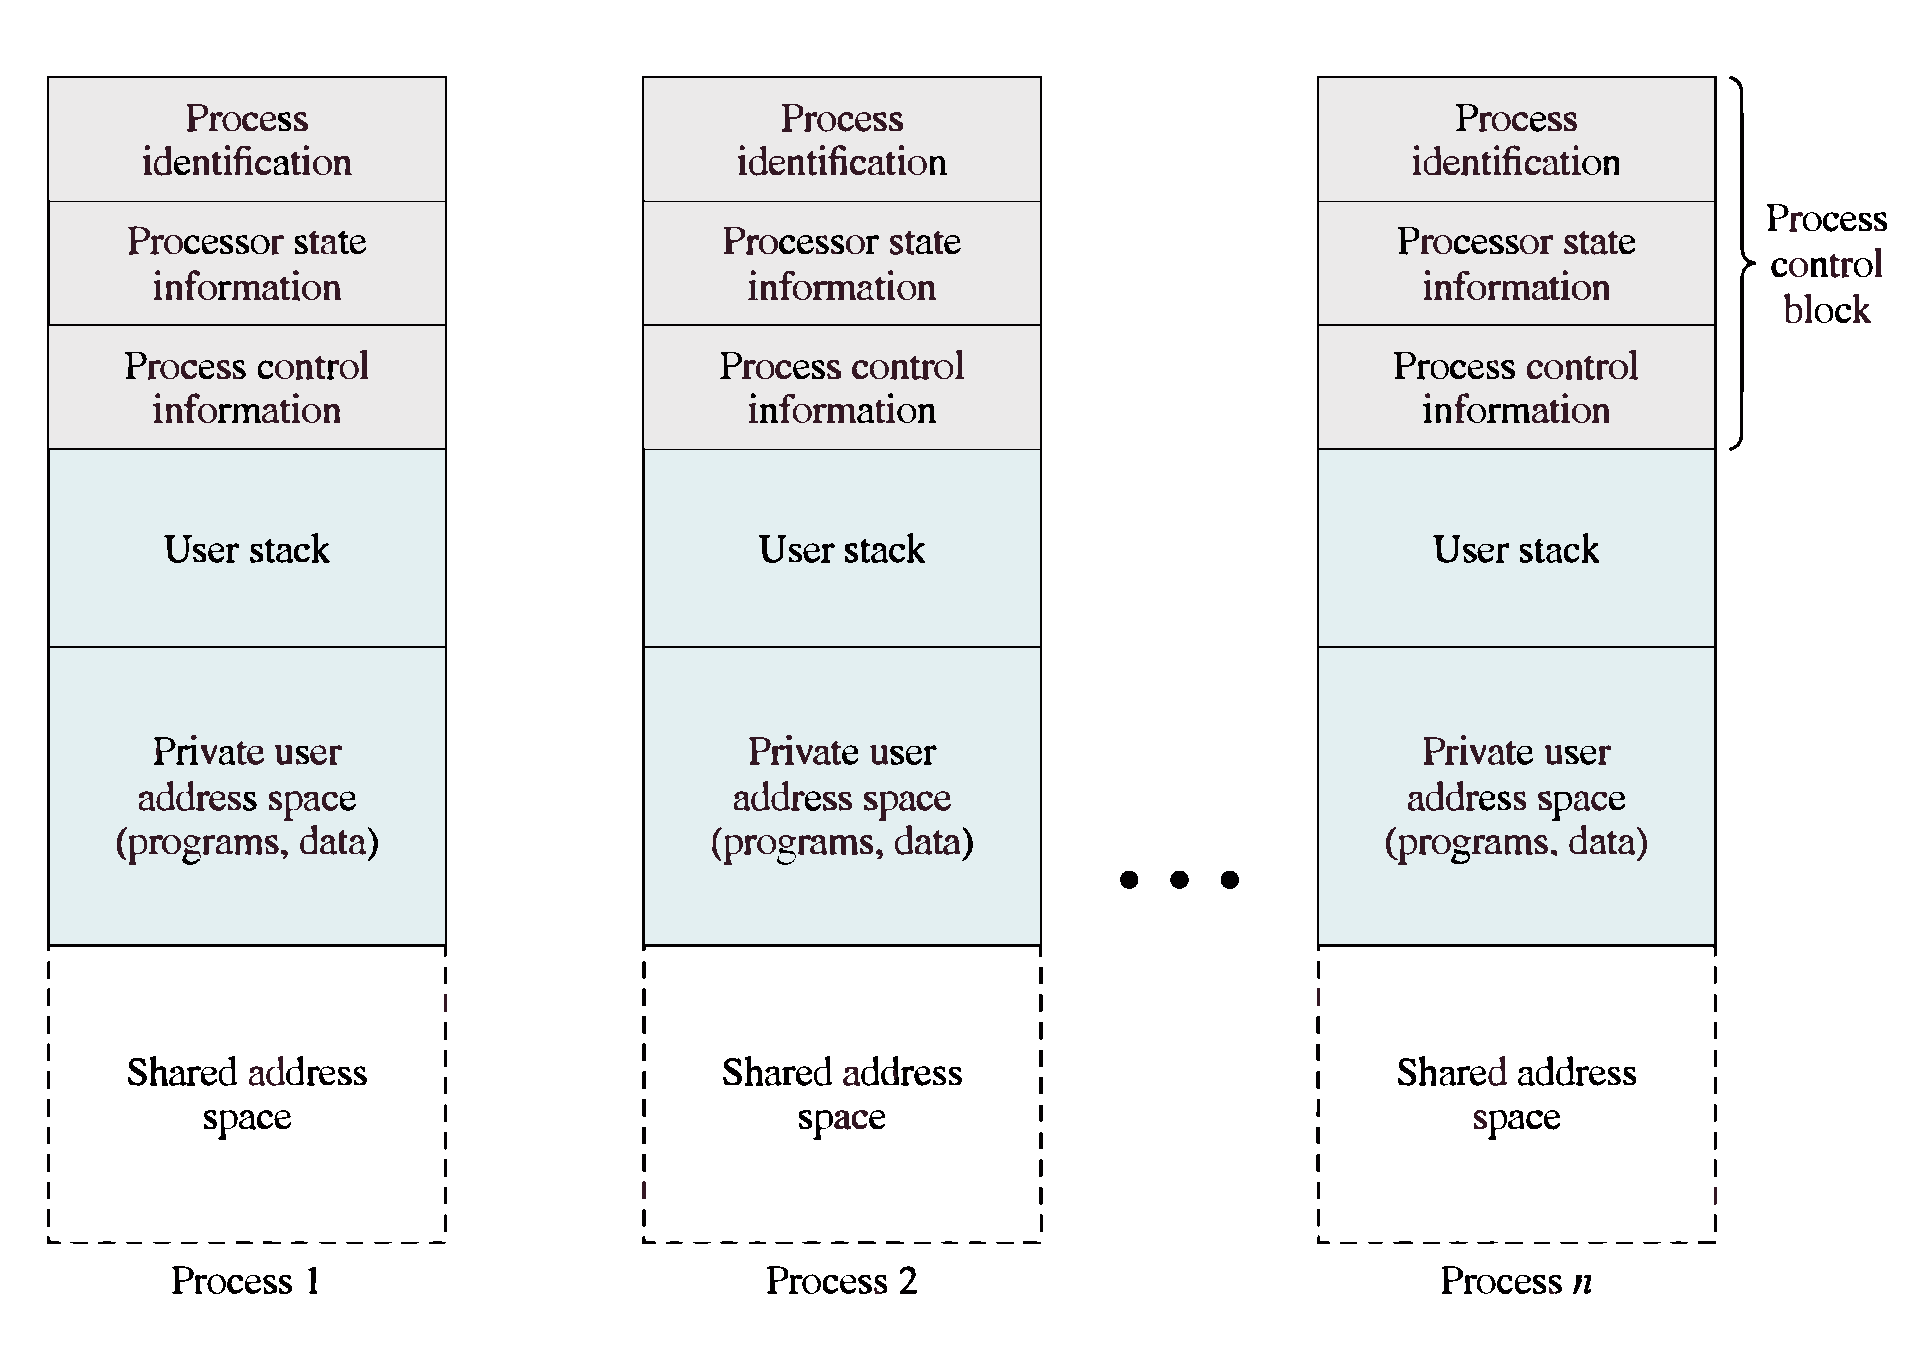
\includegraphics[width=0.90\textwidth]{assets/Proceso.eps}
    \end{center}
    \caption{Procesos en Memoria Virtual}\label{fig:1}
\end{figure}
\pagebreak

\subsection{Contexto de un proceso}
\begin{itemize}
    \item Inclute toda la informacion que el So necesita para administrar el proceso, y la CPu para ejecutarlo correctamente.
    \item Son parte del contexto, los registros de cpu, inclusive cl contador del programa, prioridad, etc.
\end{itemize}
\subsubsection{Context Switch}
\begin{itemize}
    \item Se produce cuando la cpu cambia de un proceso a otro.
    \item Se debe resguardar el contexto del proceso saliente, que pasa a espera y retornara despues a la CPU.
    \item Se debe cargar el contexto del nuevo proceso y comenzar desde la instruccion siguiente a la ultima ejecutada en dicho contexto.
    \item Es tiempo no productivo de la CPU.
    \item El tiempo que consume depende del soporte de HW.
\end{itemize}
\begin{figure}[ht]
    \begin{center}
        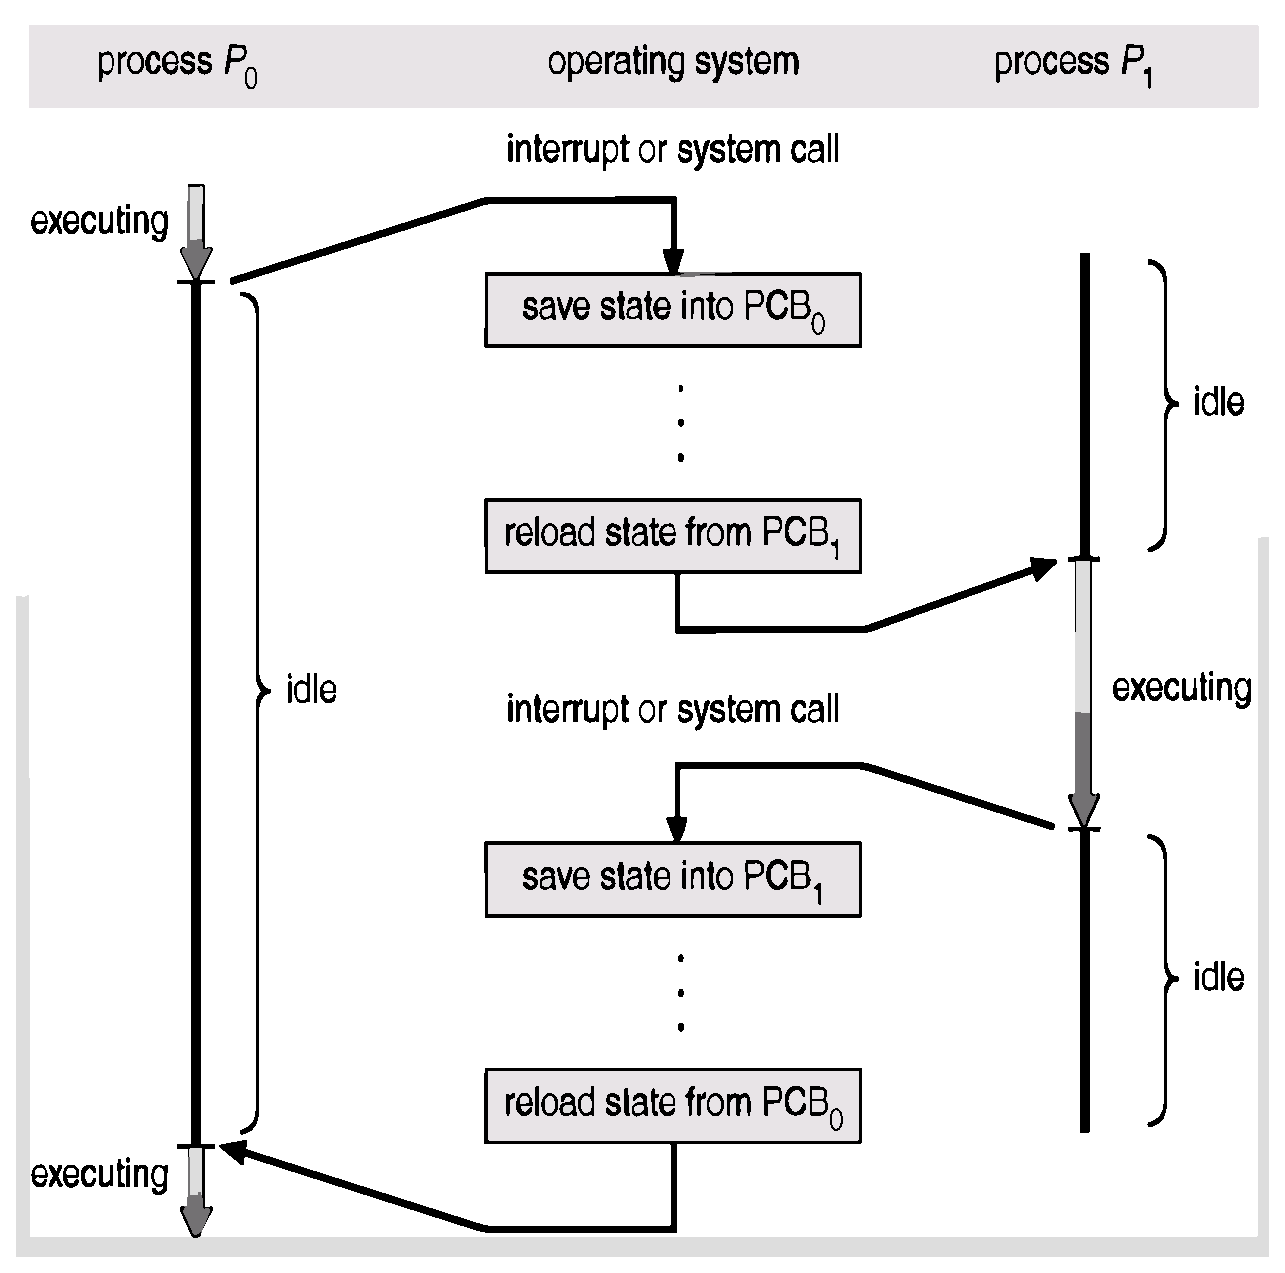
\includegraphics[width=0.65\textwidth]{assets/ContextSwitch.eps}
    \end{center}
    \caption{Context Switch}\label{fig:}
\end{figure}

\subsection{Ejecucion del Kernel}
\begin{itemize}
    \item El kernel es un conjunto de modulos de software.
    \item Se ejecuta en el procesdor como cualquier otro proceso.
    \item Existen diferentes enfoques de diseño:
\end{itemize}
\subsubsection{El kernel como entidad independiente}
\begin{itemize}
    \item El kernel se ejecuta fuera de todo proceso.
    \item El kernel se ejecuta fuera de todo proceso.
    \item Cuando un proceso es interrumpido o realiza una System Call, el contexto del proceso se salva y el control se pasa al Kernel del SO.
    \item el Kernel posee su propia region de memoria y su propio Stack.
    \item Finalizada su actividad, le devuelve el control al proceso.
    \item El kernel NO es un proceso.
    \item Se ejecuta como una entidad independiente en modo privilegiado.
\end{itemize}
\begin{figure}[h]
    \begin{center}
        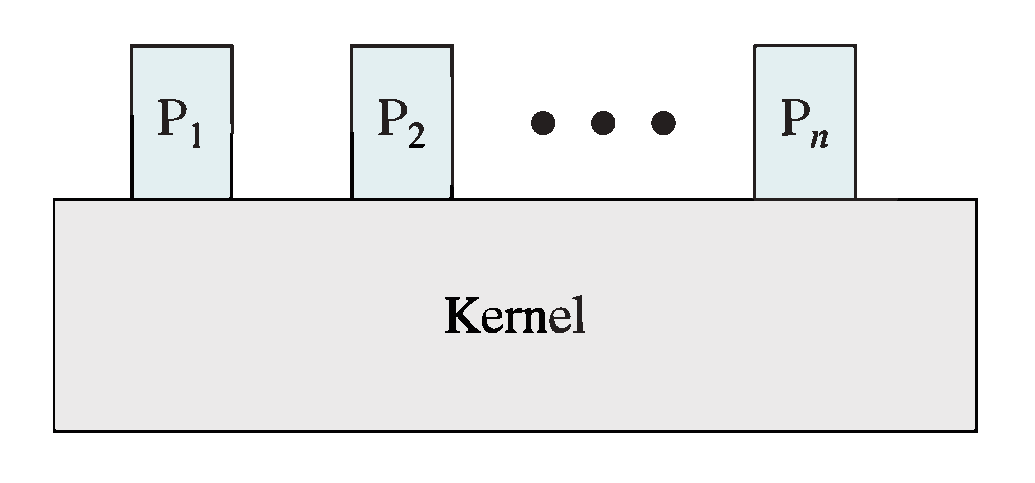
\includegraphics[width=0.45\textwidth]{assets/Kernel1.eps}
    \end{center}
    \caption{Kernel como identidad independiente}\label{fig:}
\end{figure}

\vspace{2cm}

\subsubsection{El kernel "dentro" del proceso}
\begin{itemize}
    \item El codigo del Kernel se encuentra dentro del espacio de direcciones de cada proceso.
    \item El Kernel se ejecuta en el mismo contexto que algun proceso de usuario.
    \item El Kernel se puede ver como una coleccion de rutinas que el proceso utiliza.
    \item Dentro de un proceso se encuentra el codigo del programa y el codigo de los modulos SW del SO (kernel).
    \item Cada proceso tiene un stack en modo usuario y otro en modo Kernel. 
    \item Cada interrupcion es atendida en el contexto del proceso que se encontraba en ejecucion(en modo kernel).
    \item Si el SO determina que el proceso debe seguir ejecutandose luego de atender la interrupcion, cambia a modo usuario y devuelve el control.
\end{itemize}
\vspace{2cm}
\begin{figure}[ht]
    \begin{center}
        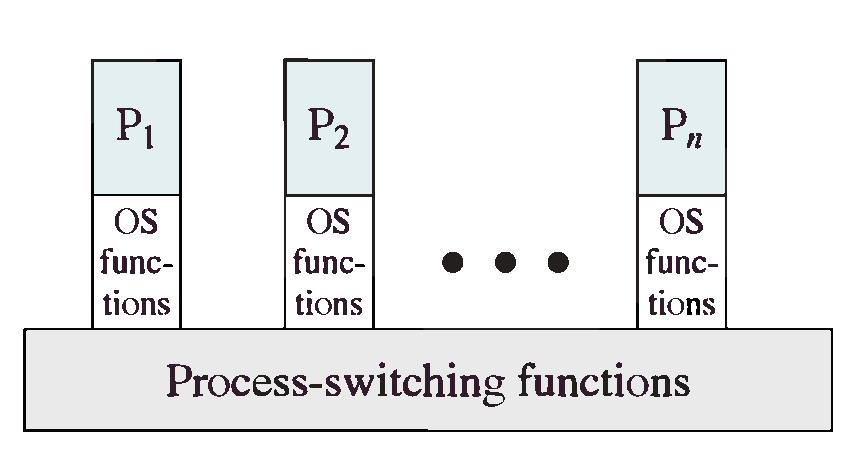
\includegraphics[width=0.50\textwidth]{assets/Kernel2.eps}
    \end{center}
    \caption{Kernel dentro del proceso}\label{fig:}
\end{figure}

\subsection{Estados de un Proceso}
En su estado de vida, un proceso pasa por diferentes estados:
\begin{itemize}
    \item \textbf{Nuevo (new)}.
    \item \textbf{Listo (ready)}.
    \item \textbf{Ejecucion (running)}.
    \item \textbf{En espera/bloqueado (waiting/blocked)}.
    \item \textbf{Terminado (terminated)}.
\end{itemize}

\begin{figure}[h]
    \begin{center}
        \includegraphics[width=0.90\textwidth]{assets/estados.png}
    \end{center}
    \caption{Estados de un proceso}\label{fig:}
\end{figure}

\pagebreak
\subsection{Colas en la planificacion de procesos}
\begin{itemize}
    \item Para realizar al planificacion, el SO utiliza la PCB de cada proceso como una abstraccion del mismo.
    \item Las PCB se enlazan en colas siguiendo un orden determinado.
\end{itemize}
\begin{figure}[h]
    \begin{center}
        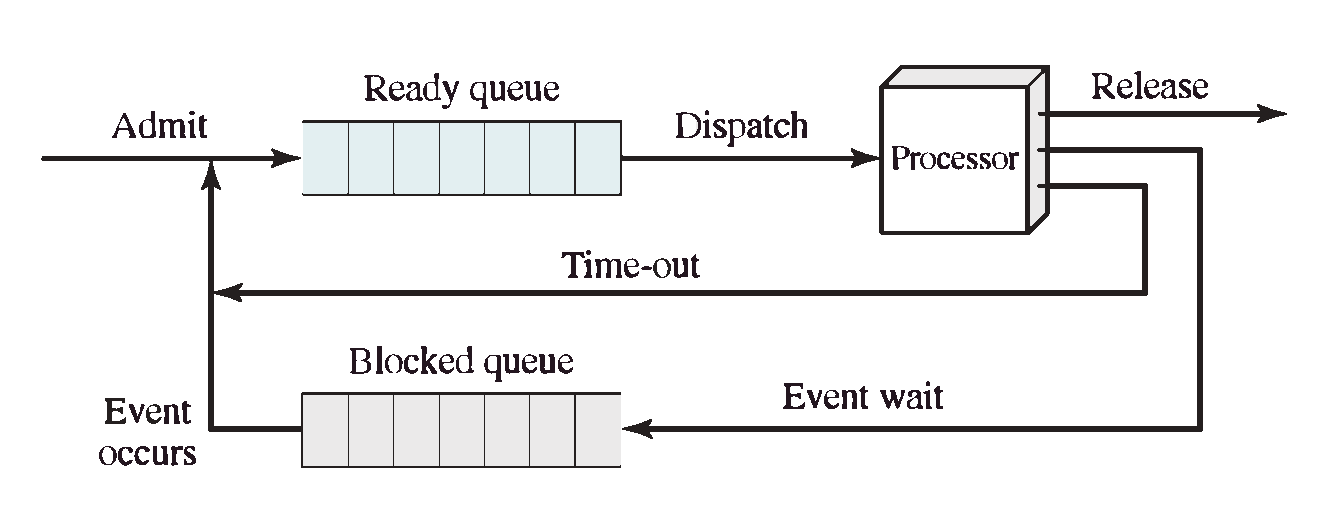
\includegraphics[width=0.75\textwidth]{assets/ProcessQueue.eps}
    \end{center}
    \caption{Colas de Planificacion}\label{fig:}
\end{figure}

\subsubsection{Modulos de la planificacion}
\begin{itemize}
    \item Son modulos de SW del Kernel que realizan distiintas tareas asociadas a la planificacion.
    \item Se ejecutan ante determinados eventos:
    \begin{itemize}
        \item Creacion/Terminacion de procesos.
        \item Eventos de sincronizacion.
        \item Finalizacion de lapso de tiempo.
        \item Etc.
    \end{itemize}
    \item Existen 3 schedulers:
        \begin{itemize}
            \item \textbf{Long Term Scheduler} 
            \item \textbf{Short Term Scheduler} 
            \item \textbf{Medium Term Scheduler} 
        \end{itemize}
    \item \textbf{Dispatcher:} realiza el cambio de contexto, cambio de modo ejecucion y despacha el proceso elegido por el Short Term.
    \item \textbf{Loader} carga en memoria el proceso elegido por el long term.
\end{itemize}
\begin{figure}[h]
    \begin{center}
        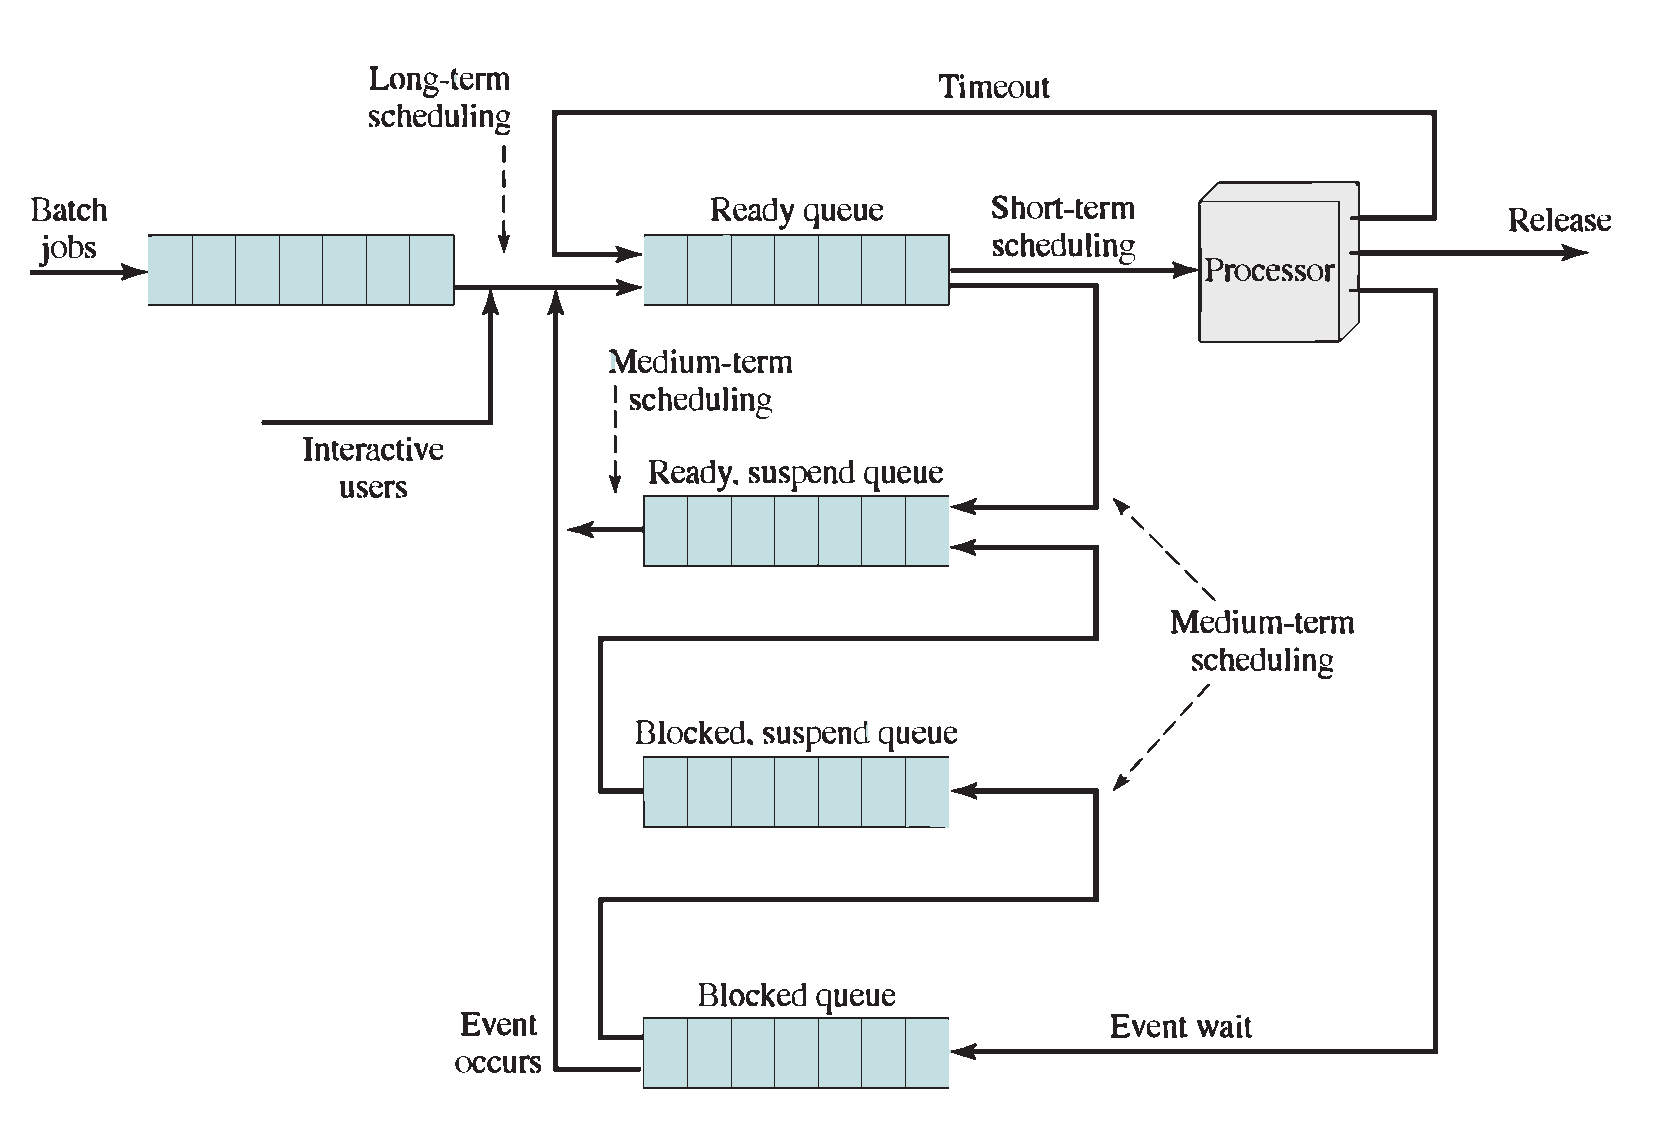
\includegraphics[width=0.90\textwidth]{assets/Schedulers.eps}
    \end{center}
    \caption{Schedulers}\label{fig:}
\end{figure}


\subsubsection{Schedulers}
\begin{itemize}
    \item \textbf{Long Term Scheduler}
        \begin{itemize}
            \item Controla el grado de multiprogramacion.
            \item Puede no existir este scheduler y absorber esta tarea el de short term.
        \end{itemize}
    \item \textbf{Medium Term Scheduler}
        \begin{itemize}
    \item Si es necesario, reduce el grado de multiprogramacion.
    \item Saca temporalmente de memoria los procesos que sea necesario para mantener el equilibrio del sistema.
\end{itemize}
\item \textbf{Short Term Scheduler}
\begin{itemize}
    \item Decide a cual de los procesos en la cola de listos se elige para que use la CPU.
    \item Terminos asociados: apropiativo, no apropiativo, algoritmo de scheduling.
\end{itemize}
\end{itemize}

\begin{figure}[ht]
    \begin{center}
        \includegraphics[width=0.50\textwidth]{assets/Schedulers2.pdf}
    \end{center}
    \caption{Schedulers}\label{fig:5}
\end{figure}

\subsection{Estados de los procesos}
\begin{itemize}
    \item \textbf{Nuevo (new):}
        \begin{itemize}
            \item Un usuario "dispara" el proceso. Un proceso es creado por otro proceso: su proceso padre.
            \item En este estado, se crean las estructuras asociadas, y el proceso queda en la cola de procesos, normalmente en espera de ser cargado en memoria.
        \end{itemize}
    \item \textbf{Listo (ready):}
        \begin{itemize}
            \item Luego que el Long Term Scheduler elige al proceo para cargarlo en memoria, el proceso queda en estado listo.
            \item El proceso solo necesita que se le asigne CPU.
            \item Esta en la cola de procesos listos (ready queue).
        \end{itemize}
    \item \textbf{Ejecucion (running):}
        \begin{itemize}
            \item El Long Term Scheduler lo eligio para asignarle CPU.
            \item Tendra la CPU hasta que se termine el periodo de tiempo asignado, termine o hasta que necesite realizar alguna operacion de E/S.
        \end{itemize}
    \item \textbf{En espera/bloqueado (waiting/blocked):}
    \begin{itemize}
        \item El proceso necesita que se cumpla el evento esperado para continuar.
        \item El evento puede ser la terminacion de una E/S solicitada, o la llegada de una senal por parte de otro proceso.
        \item Sigue en memoria, pero no tiene la CPU.
        \item Sigue en memoria, pero no tiene la CPU.
    \end{itemize}
\end{itemize}

\subsection{Comportamiento de los procesos}
\begin{itemize}
    \item \textbf{CPU-bound:} mayor parte del tiempo utilizando la CPU.
    \item \textbf{I/O bound:} mayor parte del tiempo eeperando por I/O.
\end{itemize}

\subsection{Algoritmos de Planificacion}
\begin{itemize}
    \item \textbf{Planificacion:} necesidad de determinar cual de todos los procesos que estan listos para ejecutarse, sera el proximo en ejecutarse.
    \item \textbf{Algoritmos Preemmtive:} existen situaciones que hacen que el proceso en ejecucion sea expulsado de la CPU.
    \item \textbf{Algoritmos No Preemmtive:} los procesos se ejecutan hasta que el mismo (por su propia cuenta) abandone la CPU.
\end{itemize}

\subsection{Algoritmos segun el tipo de proceso}
\subsubsection{Procesos Batch}
\begin{itemize}
    \item No existen usuarios que esperen una respuesta en la termina.
    \item Se pueden utilizar algoritmos no apropiativos.
    \item Metas propias de este tipo de algoritmos:
        \begin{itemize}
            \item Rendimiento: Maximizar  numero de trabajos por hora.
            \item Tiempo de Retorno: Minimizar los tiempos entre el comienzo y la finalizacion.
            \item El tiempo de espera se puede ver afectado.
            \item Uso de la CPU: Mantener la CPU ocupada la mayor cantidad de tiempo posible.
        \end{itemize}
\end{itemize}

\subsubsection{Procesos Interactivos}
\begin{itemize}
    \item No solo interaccion con los usuarios.
    \item Son necesarios algoritmos apropiativos para evitar que un proceso acapare la CPU.
    \item Metas propias de este tipo de algoritmos:
    \begin{itemize}
        \item Tempo de respuesta: Responder a peticiones con rapidez.
        \item Proporcionalidad: Cumplir con expectativas de los usuarios. Por ej: al poner STOP al reproductor de musica, debe dejar de ser reproducida en un tiempo corto.
    \end{itemize}
\end{itemize}

\subsection{Creacion de procesos}
\begin{itemize}
    \item Un proceso es creaado por otro proceso.
    \item Un proceso padre tiene uno o mas procesos hijos.
    \item Se forma un arbol de procesos.
    \item Actividades en la creacion:
    \begin{itemize}
        \item Crear la PCB.
        \item Asignar PID unico.
        \item Asignarle memoria para regiones.
        \item Crear estructuras de datos asociadas.
    \end{itemize}
\end{itemize}

\subsubsection{Relacion entre procesos padre e hijo}
\begin{itemize}
    \item El padre puede continuar ejcutandose concurrentemente con su hijo.
    \item El padre puede esperar a que el/los procesos hijos terminen para continuar la ejecucion.
\end{itemize}
